%--------------------
% Packages
% -------------------
\documentclass[11pt,a4paper]{article}
\usepackage[utf8]{inputenc}
\usepackage[T1]{fontenc}
%\usepackage{gentium}
\usepackage{url}
\usepackage{mathptmx} % Use Times Font
% \usepackage{wordcount}
\usepackage{pdflscape}
\usepackage[pdftex]{graphicx} % Required for including pictures
\usepackage[pdftex,linkcolor=black,pdfborder={0 0 0}]{hyperref} % Format links for pdf
\usepackage{calc} % To reset the counter in the document after title page
\usepackage[numbers]{natbib}
\usepackage{amssymb} % Required for \mathbb
\usepackage{amsmath} % Required for bmatrix environment
\frenchspacing % No double spacing between sentences
\linespread{1.2} % Set linespace
\usepackage[a4paper, lmargin=0.1666\paperwidth, rmargin=0.1666\paperwidth, tmargin=0.1111\paperheight, bmargin=0.1111\paperheight]{geometry} %margins
%\usepackage{parskip}
\usepackage{subfig}
\usepackage[all]{nowidow} % Tries to remove widows
\usepackage[protrusion=true,expansion=true]{microtype} % Improves typography, load after fontpackage is selected
\newcommand{\apjs}{ApJS}
\newcommand{\apj}{ApJ}
\newcommand{\apjl}{ApJ}
\newcommand{\mnras}{MNRAS}
\newcommand{\aap}{A\&A}
\newcommand{\aj}{AJ}
\newcommand{\nat}{Nature}
\newcommand{\bain}{Bull.~Astron.~Inst.~Netherlands} 
\newcommand{\araa}{ARA\&A}
\newcommand{\icarus}{Icarus}
\setlength{\tabcolsep}{4pt} 
\renewcommand{\arraystretch}{1}

%-----------------------
% Set pdf information and add title, fill in the fields
%-----------------------
\hypersetup{ 	
pdfsubject = {Cosmology with Gravitational Waves},
pdftitle = {Cosmology with Gravitational Waves},
pdfauthor = {Laura Just Fung (lj441)}
}
\usepackage{hyperref}
\usepackage{cleveref}

%-----------------------
% Begin document
%-----------------------
% \maketitle
\begin{document} 

\begin{center}
    \LARGE{\textbf{Gravitational Waves Coursework Assignment}}
    \\
    \Large{{Cosmology with Gravitational Waves}}
    \\
    \large{Laura Just Fung (lj441)}
    \\
    June 22, 2025
    \\
    Word count: 2142
\end{center}
\section{Introduction}
\label{sec:intro}
Gravitational wave (GW) signals are produced when two high-mass objects merge. These GW signals then propogate unimpeded by gas nor dust, and are then detected by observatories such as Advanced LIGO \citep{LIGO2015} and Advanced Virgo \citep{Acernese_2014}. In addition to the waveform of the signal encoding information about the nature of the merger, the signal's amplitude also encodes information about the luminosity distance $D_L$ to the source, allowing it to act as a standard candle. 

Additionally, as GW sources are presumably located in galaxies, if the direction to the source can be determined, it is possible to search galaxy catalogs for likely host candidates. As the redshift $z$ to these candidate galaxies are known, it is then possible to estimate the Hubble constant $H_0$. 

\section{Matched filtering}
\label{sec:matched_filtering}
\subsection{Coalescence time}
\label{sec:tc}
One way to process and analyse GW data is through matched filtering. This technique assumes that the GW signal's true waveform is known, or at least a close enough approximation to it. Using the known waveform along with the antenna response in both the plus and cross polarisations as a template applied to the received data, the signal to noise ratio (SNR) is calculated across the signal. Essentially, the template is "slid" along the signal and the SNR calculated is how much of an "agreement" there is betwwen the template and the received data. Naturally, when there is perfect overlap between the true GW signal and the template, there is a large spike in SNR. Thus, time when the SNR spikes and the time that the GW signal coalesces in the data is the same. Using this coalescence time $t_c$ in each detector, the time differences of when each detector received the signal can be calculated. Then using the known locations of each interferometer as well as which directions they are more and less sensitive to, a direction the GW source can be determined. 

As the antenna response from each interferometer depends on the assumed sky area the signal is originating from, the SNR for each interferometer H1, L1, and V1 was calculated in a grid of 10 $\mathrm{deg}^2$ segments spanning the full sky area. It was assumed that the antenna response did not vary significantly over the considered time segment, 4 seconds from GPS time 1126259460.4 s, thus the antenna response was calculated at the midpoint time of the segment for each interferometer. The SNR was then calculated for each interferometer in each segment, and the maximum SNR across all interferometers was used to determine the most likely sky area the signal originated from. The full-width half-maximum (FWHM) of the SNR distribution was then used to determine the uncertainty on the coalescence times $t_c$ for each interferometer, shown in Table~\ref{tab:tcs}. The SNR distributions for each interferometer are shown in Fig.~\ref{fig:snr_distributions}.

\begin{figure}
    \includegraphics[width=\columnwidth, keepaspectratio]{../figures/SNR_HLV.png}
    \caption{SNR distributions for each interferometer H1 (2nd panel, blue), L1 (3rd panel, yellow), and V1 (4th panel, pink). The SNR is calculated in 10 $\mathrm{deg}^2$ segments across the sky area. The shaded areas show the 1 $\sigma$ uncertainty on the coalescence time $t_c$, which is used to determine the uncertainty on the coalescence time $t_c$ for each interferometer. The first panel shows all three interferometers' SNR distributions.}
    \label{fig:snr_distributions}
\end{figure}

\begin{table}[h]
    \centering
    \begin{tabular}{cc}
    Interferometer & Coalescence time from 1126259460.4s $t_c$ (s) \\
    $t_c^{(H1)}$ & 2.017 $\pm$ 0.001 \\
    $t_c^{(L1)}$ & 2.010 $\pm$ 0.002 \\
    $t_c^{(V1)}$ & 2.009 $\pm$ 0.001 \\
    \end{tabular}
    \caption{Coalescence times from 1126259460.4s for each interferometer H1, L1, and V1 and their uncertainties.}
    \label{tab:tcs}
\end{table}

The relative time delays for the interferometer pairs HL, HV, and VL are shown in Table~\ref{tab:tds}.

\begin{table}[h]
    \centering
    \begin{tabular}{cc}
    Interferometer pairs & Time delay (s) \\
    $t_c^{(H1)} - t_c^{(L1)}$ & 0.007 $\pm$ 0.002 \\
    $t_c^{(H1)} - t_c^{(V1)}$ & 0.008 $\pm$ 0.002 \\
    $t_c^{(V1)} - t_c^{(L1)}$ & 0.001 $\pm$ 0.002 \\
    \end{tabular}
    \caption{Relative time delays for interferometer pairs HL, HV, and VL and their uncertainties.}
    \label{tab:tds}
\end{table}

It makes sense to consider V1 separately from H1 and L1 because H1 and L1 LIGO are located in the United States and are managed by the LIGO Scientific Collaboration while V1 is located in Italy and managed by the European Gravitational Observatory \citep{LIGO2015, Acernese}. The different geographical locations as well as the independent design and management, means that V1 will provide dissimilar time delays compared to H1 and L1 as well as different antenna responses to sky areas. Additionally, the V1 interferometer can also provide additional independent confirmation of a GW signal. This allows for better triangulation of the GW source location and improved sky localization beyond what is possible with just the HL pair.

\subsection{Sky map}
\label{sec:skymap_mf}
Using the relative time delays and their uncertainties, as well as the known location of each interferometer on the Earth, the direction to the GW source can be estimated. This was done by creating a time delay map for the interferometer pairs using the \texttt{time\_delay\_from\_geocenter} method from \texttt{bilby}. Then, by comparing the delay map to the calculated time delays from Sec~\ref{sec:tc}, a probability map was calculated using Eq.~\ref{eq:prob}:

\begin{equation}
    L = \exp{\frac{-0.5(D^i-t_d^i)^2}{{\sigma^i}^2}},
    \label{eq:prob}
\end{equation}

where $D^i$ is the delay map for each interferometer pair, $t_d^i$ is the calculated time delay for each interferometer pair, and $\sigma^i$ is the uncertainty on the time delay for each interferometer pair. The resulting map for the HL pair is shown in Fig.~\ref{fig:skymap_hl_mf}. As seen in the figure, the likely sky area of the GW source is quite large and uncertain, covering 8472.82 $\mathrm{deg}^2$, or about 20.54\% of the sky.

\begin{figure}
    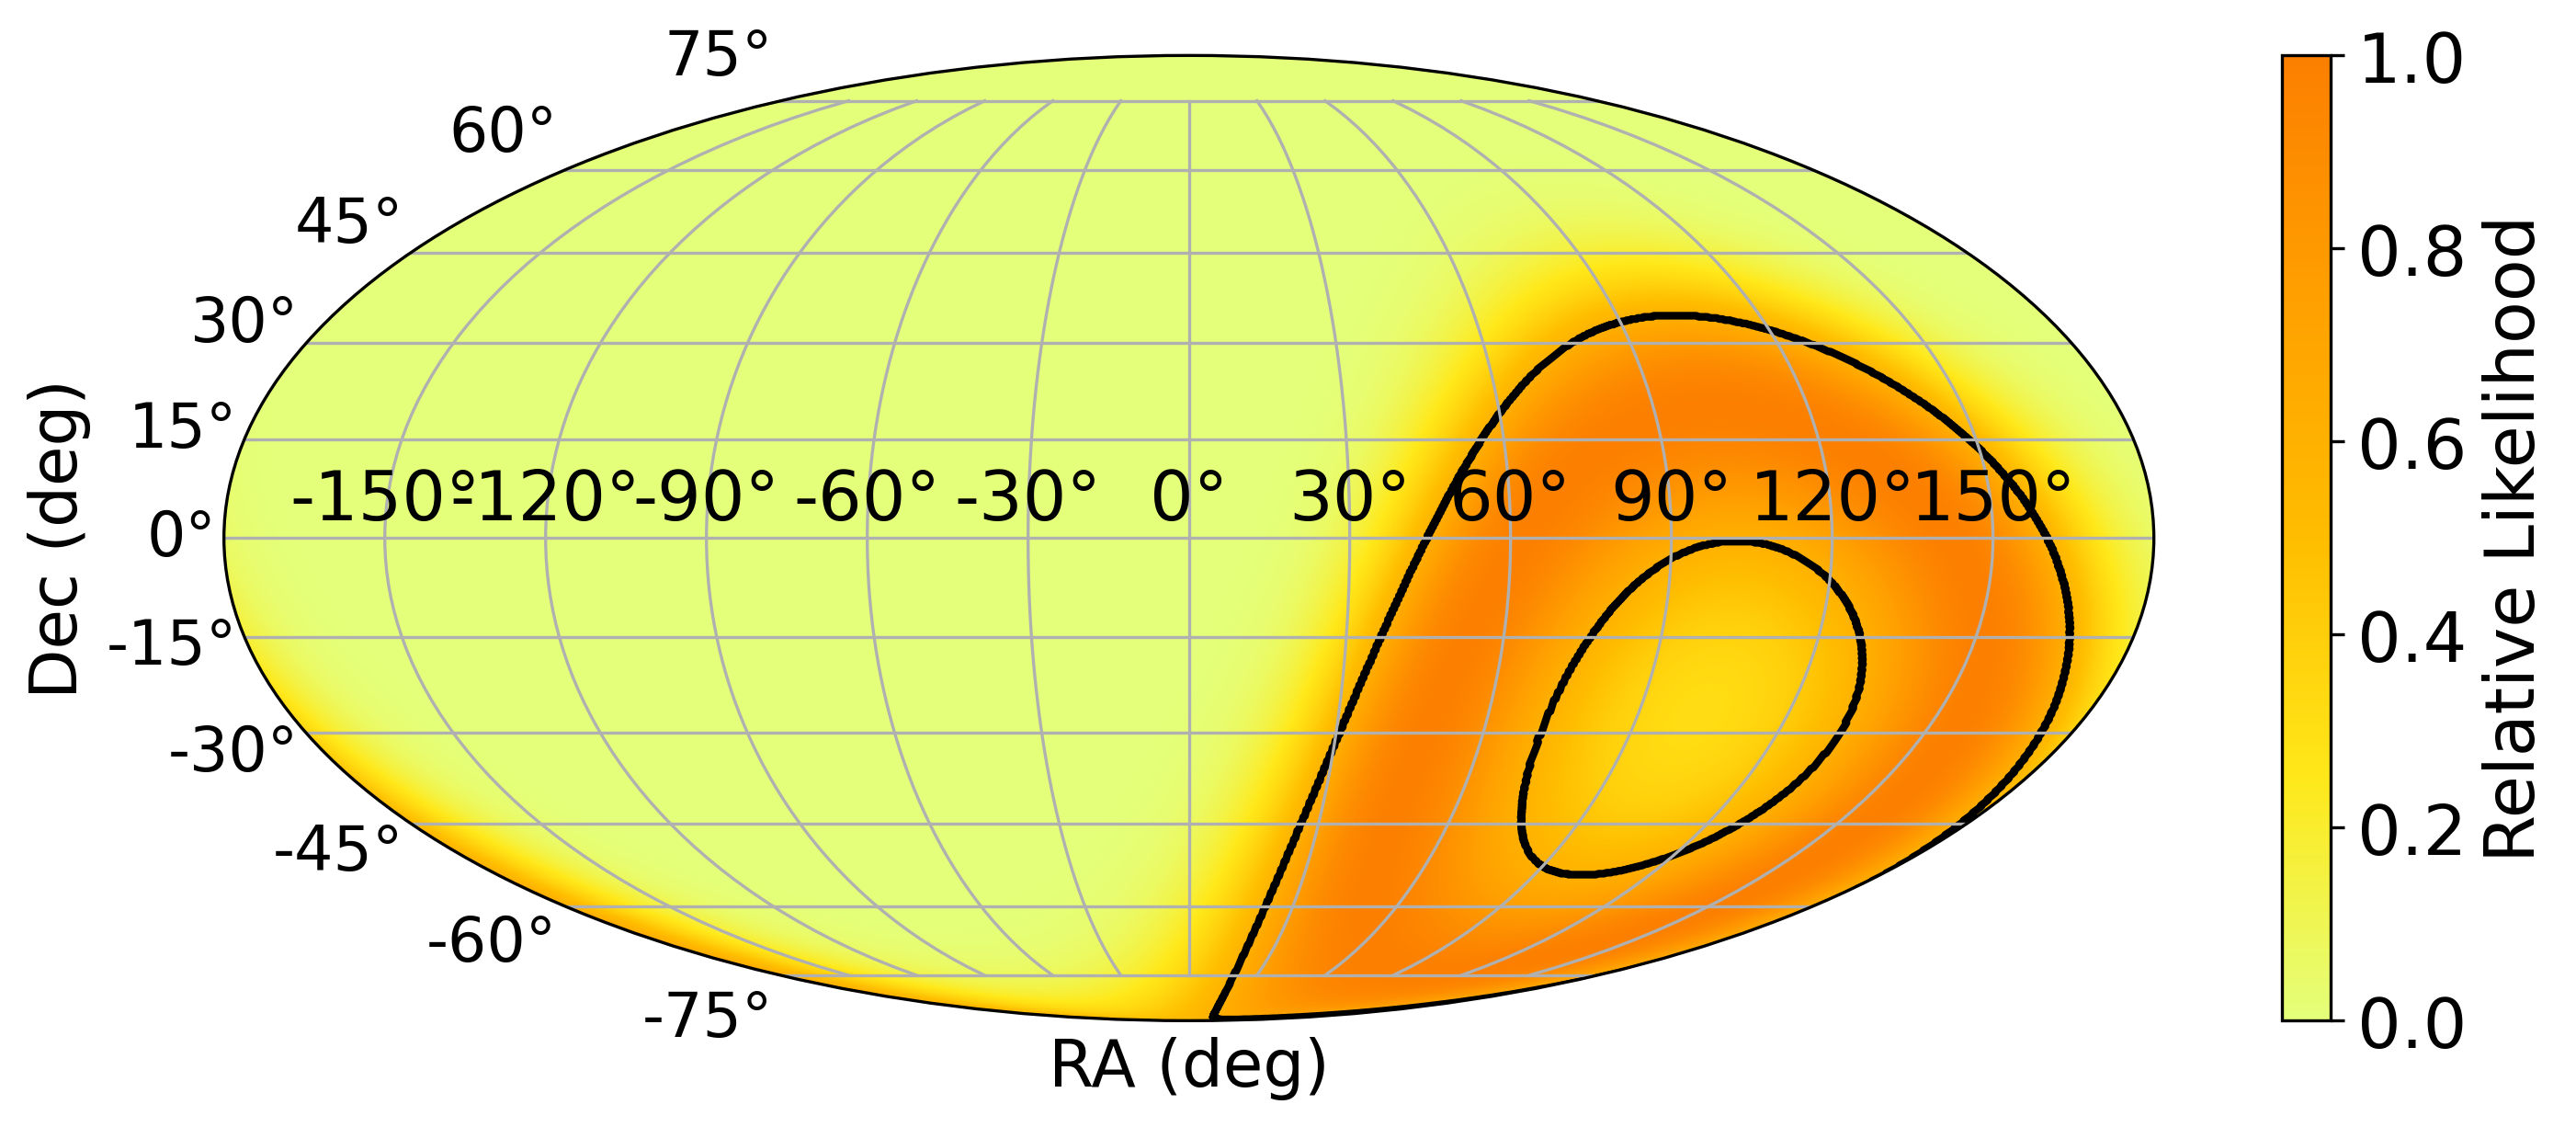
\includegraphics[width=\columnwidth, keepaspectratio]{../figures/detector_skymap_HL.png}
    \caption{Probability sky map for the HL interferometer pair using matched filtering. The color scale shows the probability of the GW source being in each sky area.}
    \label{fig:skymap_hl_mf}
\end{figure}

When including the Virgo V1 interferometer and thus the HV and VL pairs, the uncertainty on the sky area is reduced to 0.85\% of the sky, or 351.39 $\mathrm{deg}^2$. The resulting sky map showing all three interferometer pair likely areas are shown in Fig.~\ref{fig:skymap_hlv_mf}. The reduction in likely sky area and thus improvement of the localization of the GW source due to the inclusion of the Virgo V1 interferometer is 95.85\%.

This improvement is because V1 provides additional constraints on the relative time delays. As V1 is located in Italy while H1 and L1 are located in the United States, the differences in signal arrival times allows for better triangulation of the GW source location.

\begin{figure}
    
\includegraphics[width=\columnwidth, keepaspectratio]{../figures/detector_skymap_intersection.png}
    \caption{Sky map for the three interferometer pairs using matched filtering. Top: masks of likely area for interferometer pairs HL (blue), HV (green), and VL (yellow). The red contour highlights the intersection of all three masks. Bottom: the combined probability sky map for all three interferometer pairs. The color scale shows the probability of the GW source being in each sky area.}
    \label{fig:skymap_hlv_mf}
\end{figure}

\clearpage
\section{Bayesian inference}
\label{sec:bayesian}
In addition to matched filtering, Bayesian inference can also be used to determine the characteristics of the GW source including the sky location, luminosity distance, coalescence time, and polarisation angle $\psi$.

Using the \texttt{bilby} library's functions to calculate the time delays between the detectors and the geocenter as well as the antenna patterns $F_\mathrm{+}$ and $F_\times$, Bayesian inference was performed on the GW signal to determine the posterior distributions of the source parameters. The likelihood function used for this analysis is given by Eq.~\ref{eq:likelihood}:

\begin{equation}
    \log \mathcal{L}(\vec{\theta}) = 
    -2 \sum_{\text{IFOs}} \sum_{f}
    \left[
    \frac{\left| h_{\text{obs}}(f) - \frac{1}{D_L} \left( {F_+} h_+(f) + {F_\times} h_\times(f) \right) e^{-2\pi i f (t_c + \Delta t)} \right|^2}{\text{ASD}(f)^2}
    \right] \Delta f
    \label{eq:likelihood}
\end{equation}    

where $\vec{\theta}$ represents the parameters $(\alpha, \delta, \psi, t_c, D_L)$, $h_{\text{obs}}(f)$ is the observed data in the frequency domain, $F_+$ and $F_\times$ are the plus and cross antenna reponses for each interferometer, $h_+(f)$ and $h_\times(f)$ are the plus and cross polarisations of the GW signal in the frequency domain, $\Delta t$ is the time delay between the interferometer and the geocenter for each interferometer, and $\text{ASD}(f)$ is the amplitude spectral density for the signal received in each interferometer. 

The priors used for the analysis were chosen to be uniform for RA, solid angle (Dec), coalescence time, and polarisation angle while log-uniform over luminosity distance. Their ranges are shown in Table~\ref{tab:priors}.

\begin{table}[h]
    \centering
    \begin{tabular}{cc}
    Parameter & Value range \\
    RA ($\alpha$, rad) & [0, $2\pi$] \\
    Dec ($\delta$, rad) & $\arcsin(-\frac{\delta}{2}-1)$ \\
    Polarisation angle ($\psi$, rad) & [0, $2\pi$] \\
    Geocentric coalescence time from 1126259460.4 ($t_c^{geo}$, s) & [0, 4] \\
    Luminosity distance ($D_L$, Mpc) & [$10^{-4}$, $10^5$] \\
    \end{tabular}
    \caption{Prior distributions for each gravitational-wave parameter. The RA and Dec are in radians, the polarisation angle is in radians, the coalescence time is in seconds, and the luminosity distance is in Gigaparsecs. The Dec prior is calculated using the inverse sine function to ensure that the prior is uniform over the solid angle.}
    \label{tab:priors}
\end{table}


Using the \texttt{dynesty} package to perform the nested sampling, the posterior distributions for the parameters were calculated. The posterior results for the HL interferometer pair after resampling for equal weight are shown in Fig.~\ref{fig:posterior_hl}. Note that in this projection, RA increases leftward, 'flipping' the map compared to Section~\ref{sec:skymap_mf}. The Mollweide projected RA and Dec posteriors are shown in Fig.~\ref{fig:sky_hl}. As seen, the posterior RA distribution is quite wide, encompassing around 60 ${\deg}^2$ while the posterior Dec distribution is more constrained, encompassing around 30 ${\deg}^2$. 

The median location of the source is at RA = $2.477^{+0.164}_{-0.510}$ rad and Dec = $-1.123^{+0.214}_{-0.137}$ rad. The 1D marginalised distribution of the luminosity distance $D_L$ is shown in Fig.~\ref{fig:luminosity_distance}. The median luminosity distance is $1.02 \pm 0.03$ Gpc.
\begin{figure}
    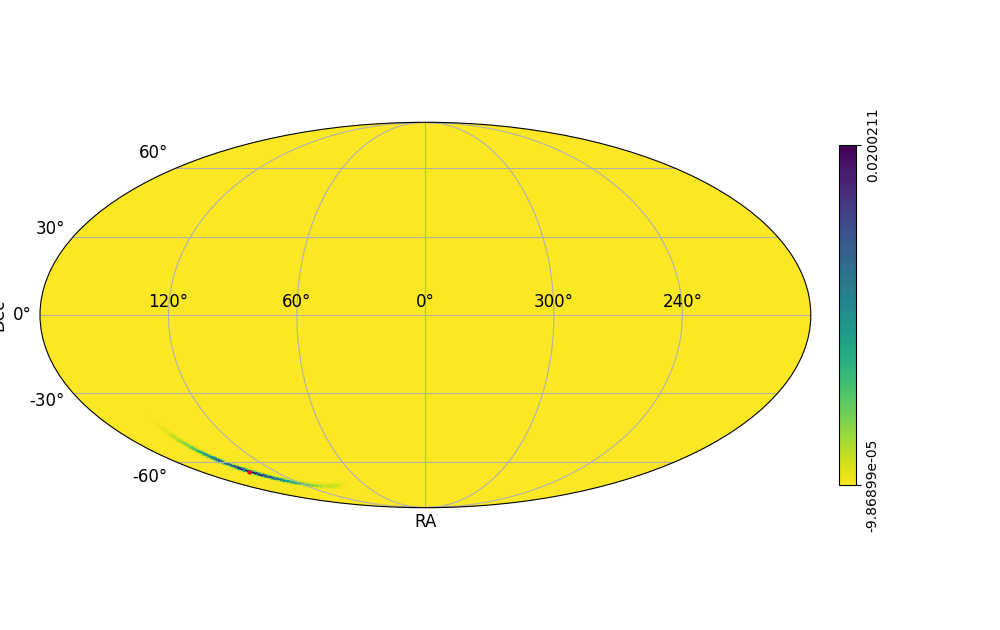
\includegraphics[width=\columnwidth, keepaspectratio]{../figures/posterior_map_HL.png}
    \caption{Mollweide projection of the sky showing the normalised posterior distribution for the HL interferometer pair. The color scale shows the probability density of the GW source being in each sky area. The red dot indicates the median position of the source.}
    \label{fig:sky_hl}
\end{figure}

Fig.~\ref{fig:hl_compare} compares the posterior distribution of the RA and Dec coordinates from the Bayesian inference method to the matched filtering method. It is clear that the Bayesian inference method provides a much more precise localization of the GW source, with the resampled posterior distribution enclosing only 0.23\% of the sky, or 93.16 $\mathrm{deg}^2$.

\begin{figure}
    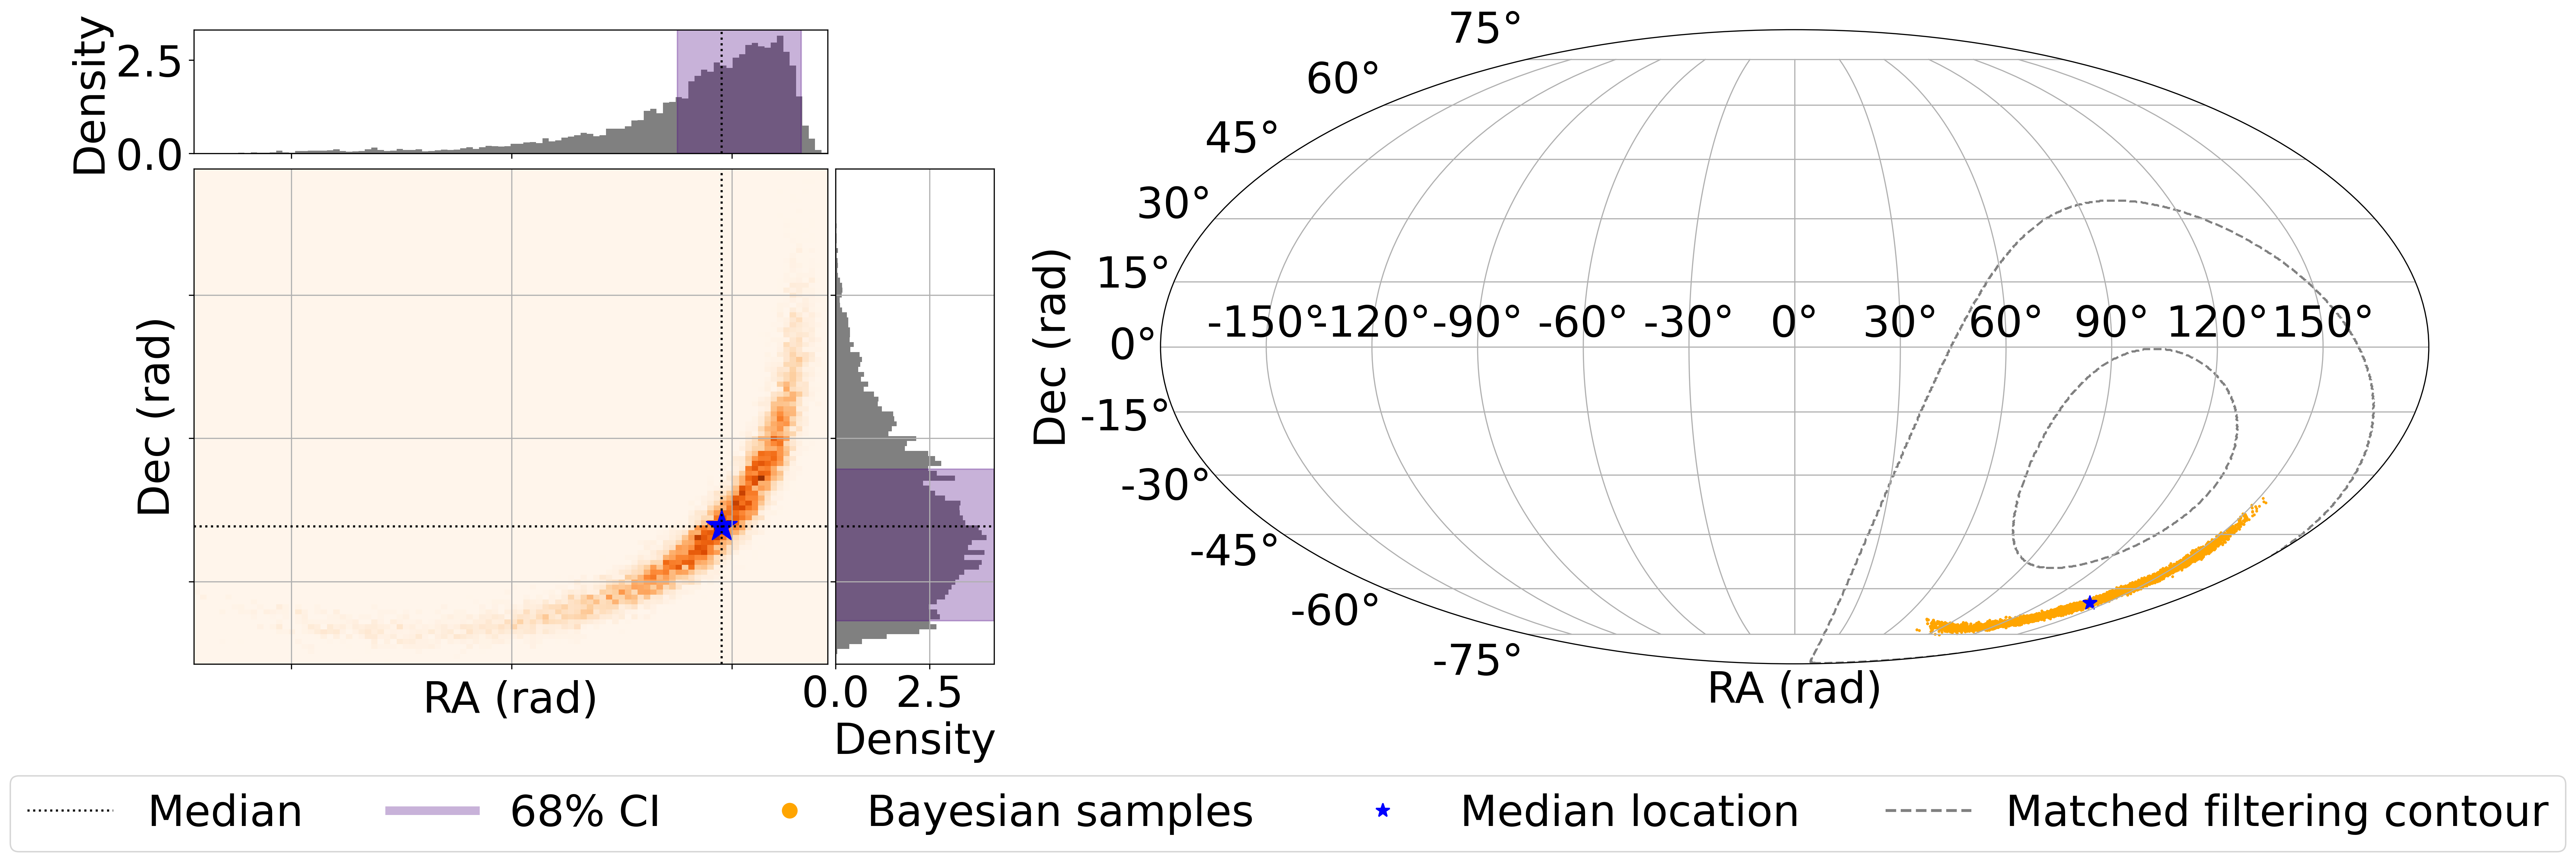
\includegraphics[width=\columnwidth, keepaspectratio]{../figures/radec_posterior_HL.png}
    \caption{Left: RA and Dec posterior distribution from the Bayesian inference method with 1D marginalisations of the RA and Dec coordinates. The shaded area (purple) indicates the 68\% credible interval while the dotted lines indicate the median of both the RA and Dec distributions. Right: Comparison of the posterior distribution of the RA and Dec coordinates from the Bayesian inference method to the matched filtering method. The grey contour shows the matched filtering enclosed area while the orange scatter points show the posterior distribution from the Bayesian inference method. The blue star indicates the median location of the source.}
    \label{fig:hl_compare}
\end{figure}
\clearpage
Including the Virgo V1 interferometer in the Bayesian inference method, the corner plot of the posterior distributions is shown in Fig.~\ref{fig:posterior_hlv}. The Mollweide projected RA and Dec posteriors of the resampled distribution are in Fig.~\ref{fig:sky_hlv}. The 1D marginalised distribution of the luminosity distance $D_L$ is shown in Fig.~\ref{fig:luminosity_distance}. The median luminosity distance is $1.02 \pm 0.03$ Gpc, which is consistent with the HL interferometer pair result. Fig.~\ref{fig:hlv_compare} compares the posterior distribution of the RA and Dec coordinates from the Bayesian inference method to the matched filtering method. 

The resampled posterior distribution encloses only 0.01\% of the sky, or 5.04 $\mathrm{deg}^2$. Thus, including the Virgo V1 interferometer in the analysis provides a significant improvement in the localization of the GW source, with an improvement of 98.75\% over the HL interferometer pair matched filtering method.

Table~\ref{tab:areas} summarises the sky areas for the matched filtering and Bayesian inference methods for both the HL and HLV interferometer pairs. Table~\ref{tab:params} summarises the median and 1$\sigma$ uncertainties for the parameters obtained from the Bayesian inference method for both the HL and HLV interferometer pairs.

\begin{figure}
    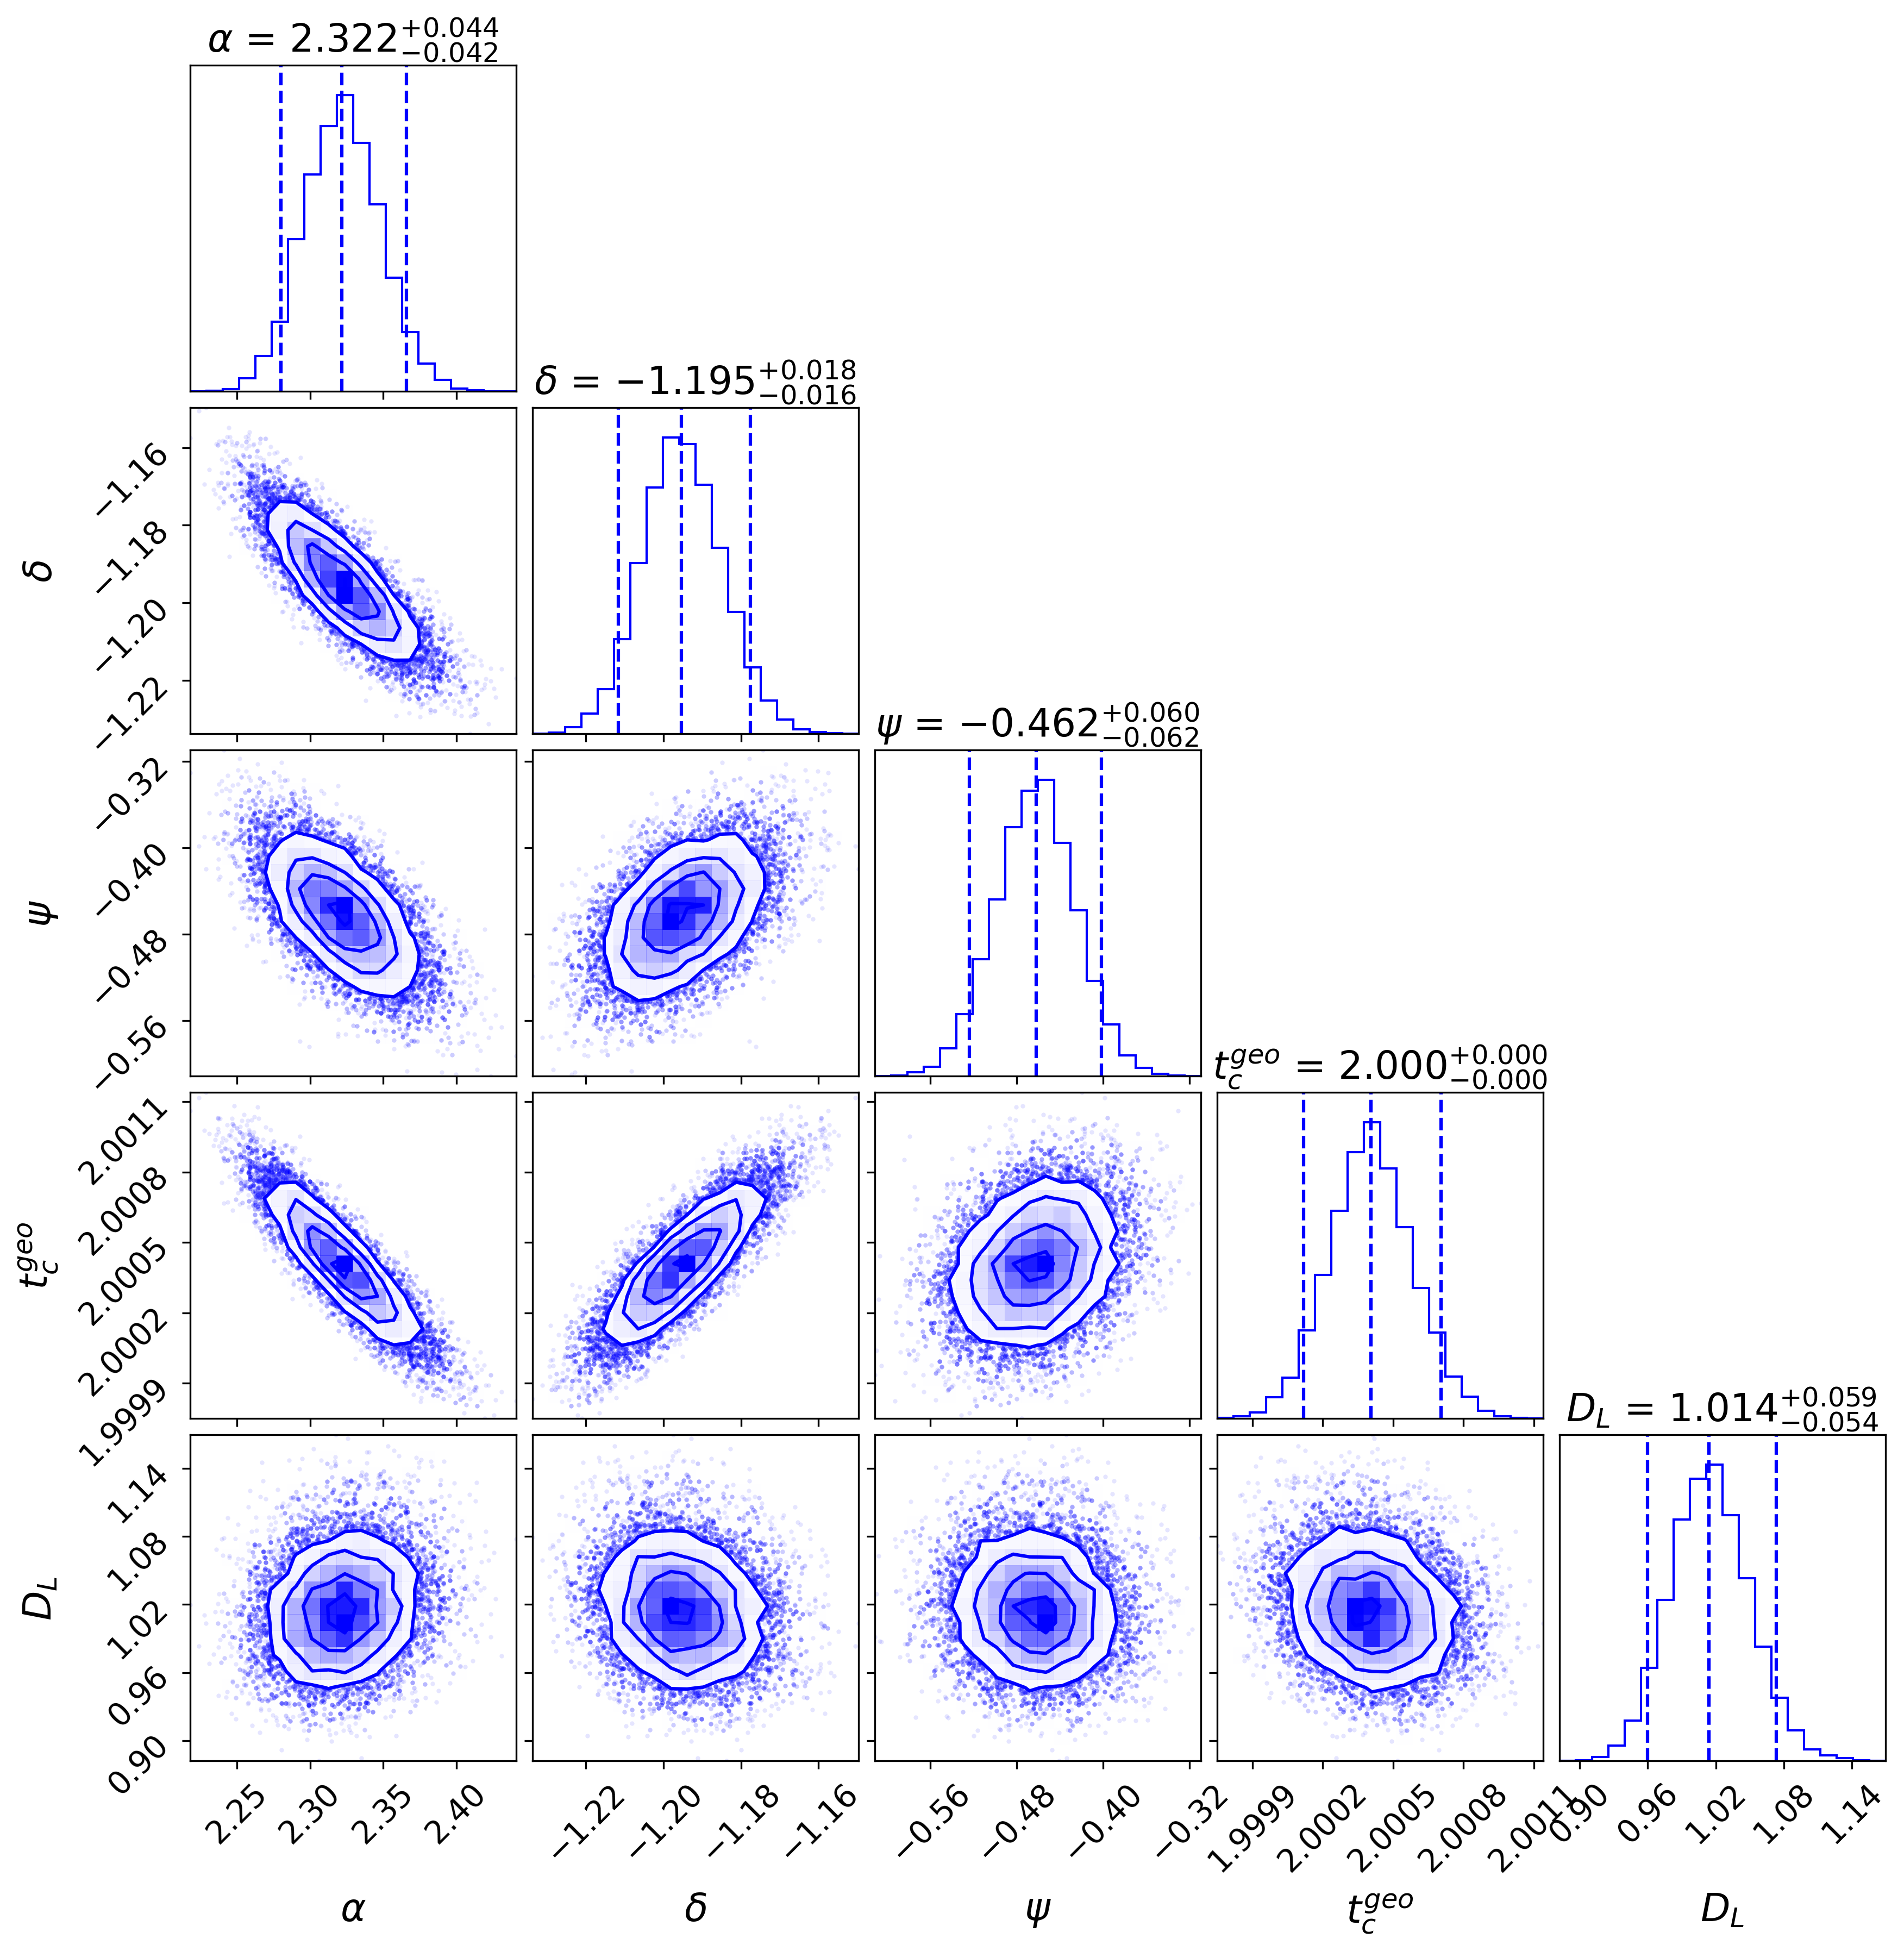
\includegraphics[width=\columnwidth, keepaspectratio]{../figures/corner_HLV.png}
    \caption{Corner plot showing the posterior distributions for the HL and V1 interferometer pair obtained via Bayesian inference. From left to right, the parameters are the right ascension ($\alpha$), declination ($\delta$), polarisation angle ($\psi$), geocentric coalescence time ($t_c^{geo}$), and luminosity distance ($D_L$). The 2D contour plots show the 1$\sigma$ (68.3\%) and 2$\sigma$ (95.4\%) credible regions. The diagonal plots display the marginalized posterior distributions for each parameter, with vertical lines indicating the 5th, 50th (median), and 95th percentiles.}
    \label{fig:posterior_hlv}
\end{figure}

\begin{figure}
    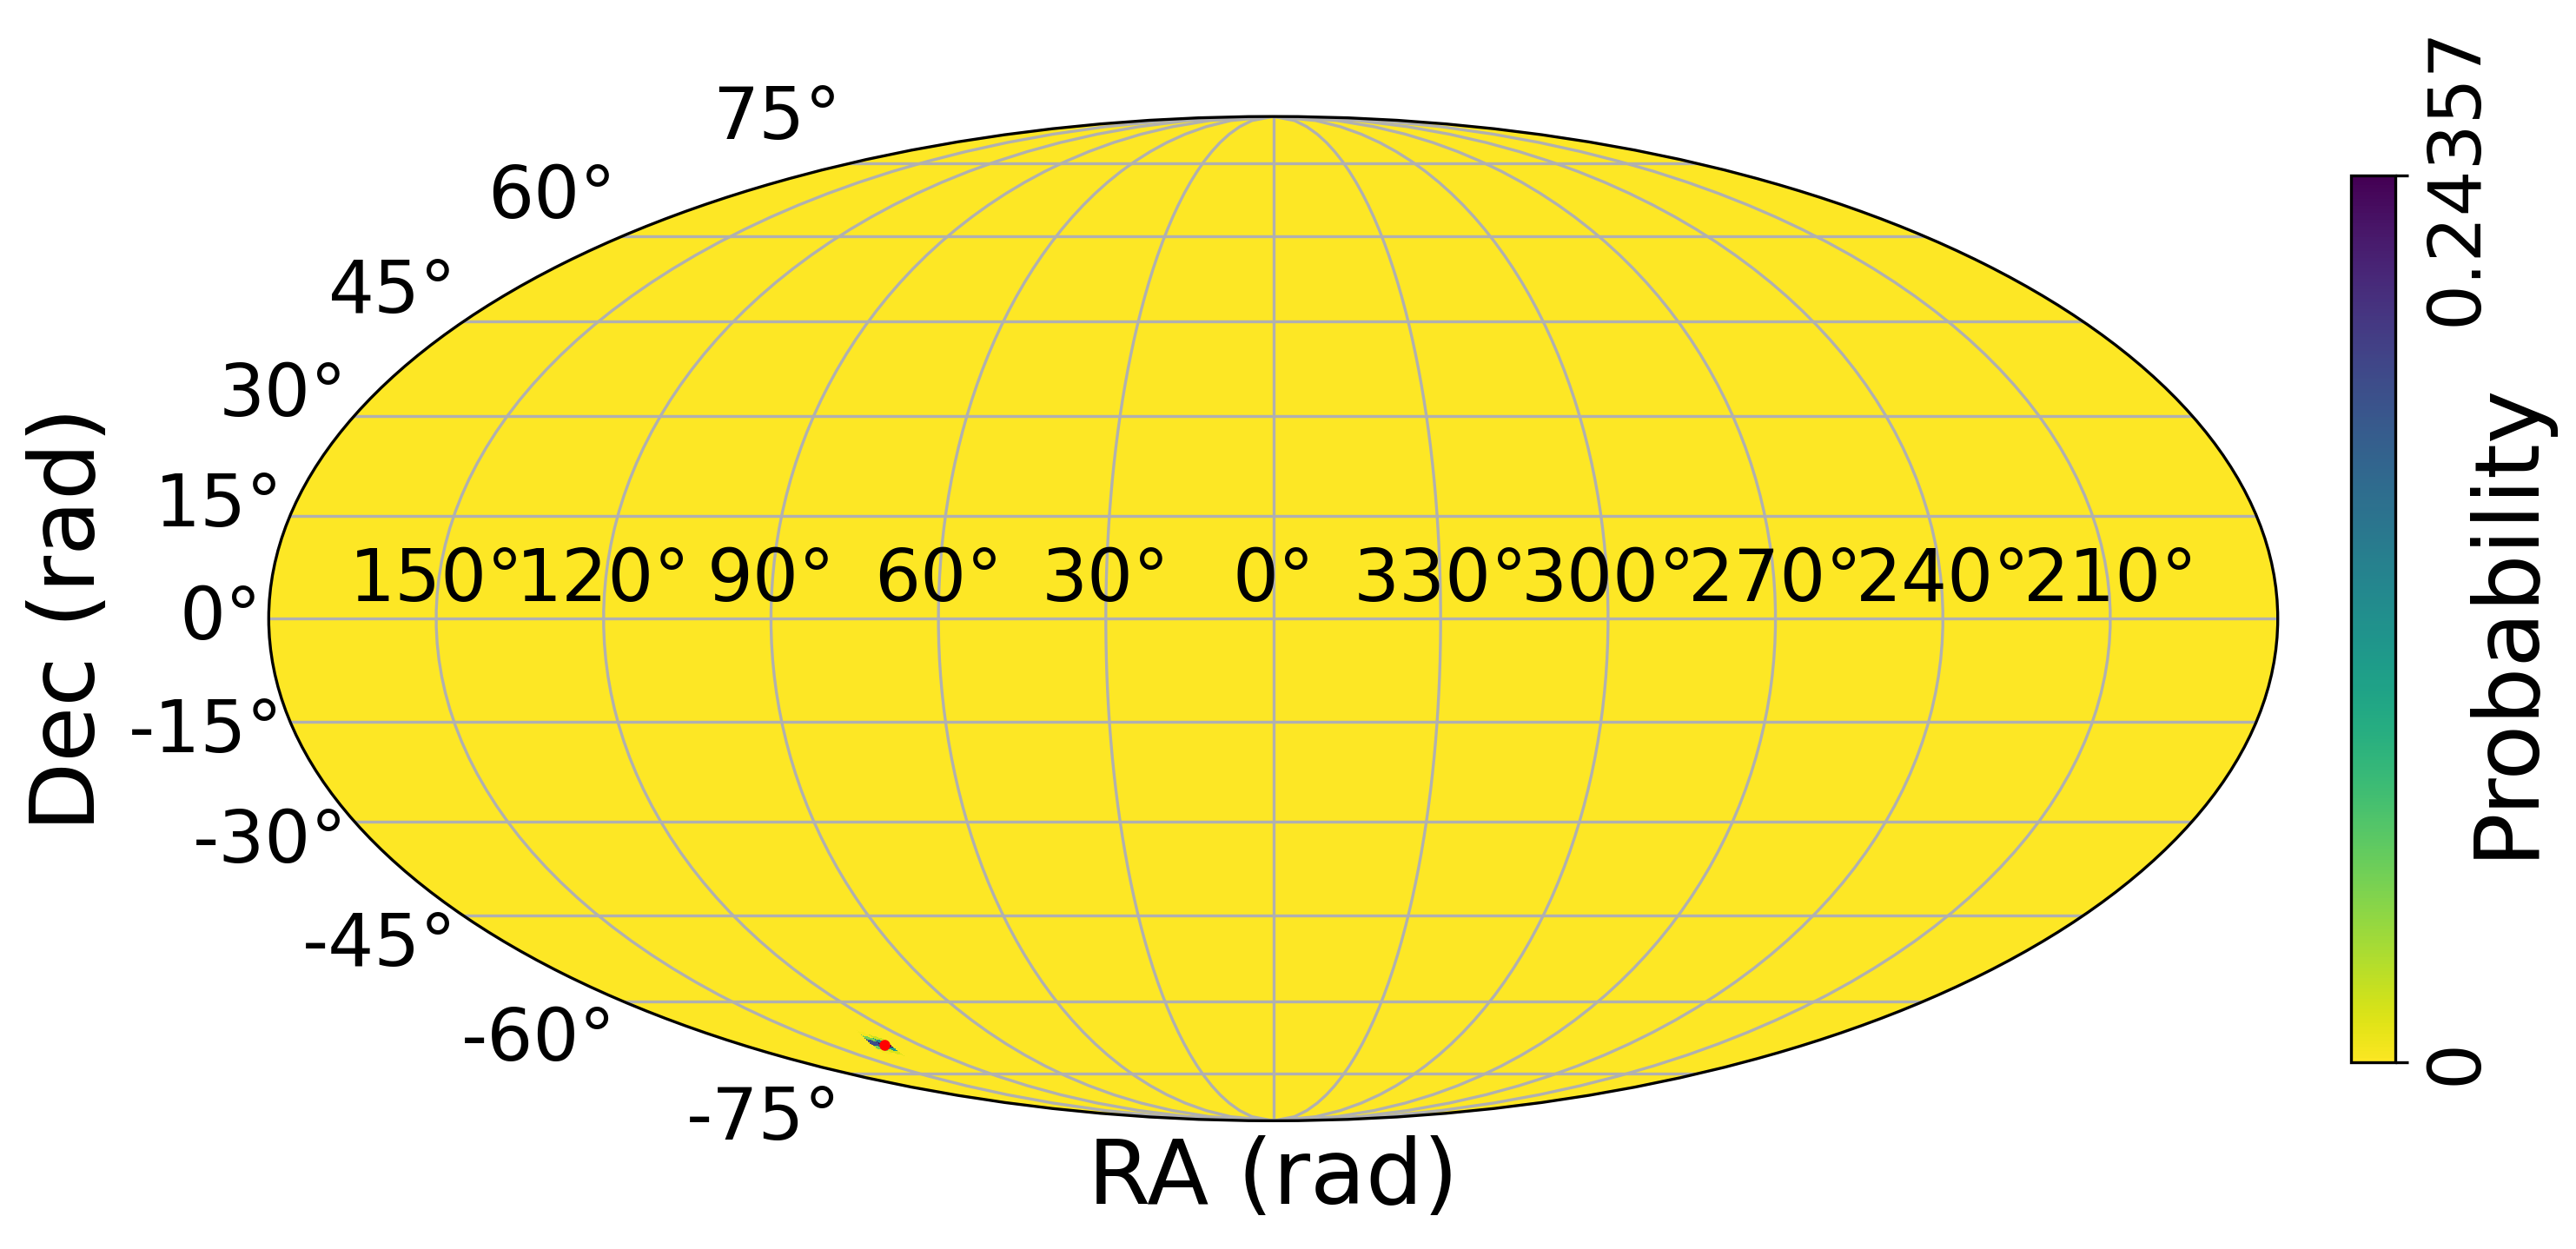
\includegraphics[width=\columnwidth, keepaspectratio]{../figures/posterior_map_HLV.png}
    \caption{Mollweide projection of the sky showing the normalised posterior distribution for the HL and V1 interferometer pair. The color scale shows the probability density of the GW source being in each sky area. The red dot indicates the median position of the source.}
    \label{fig:sky_hlv}
\end{figure}

\begin{figure}
    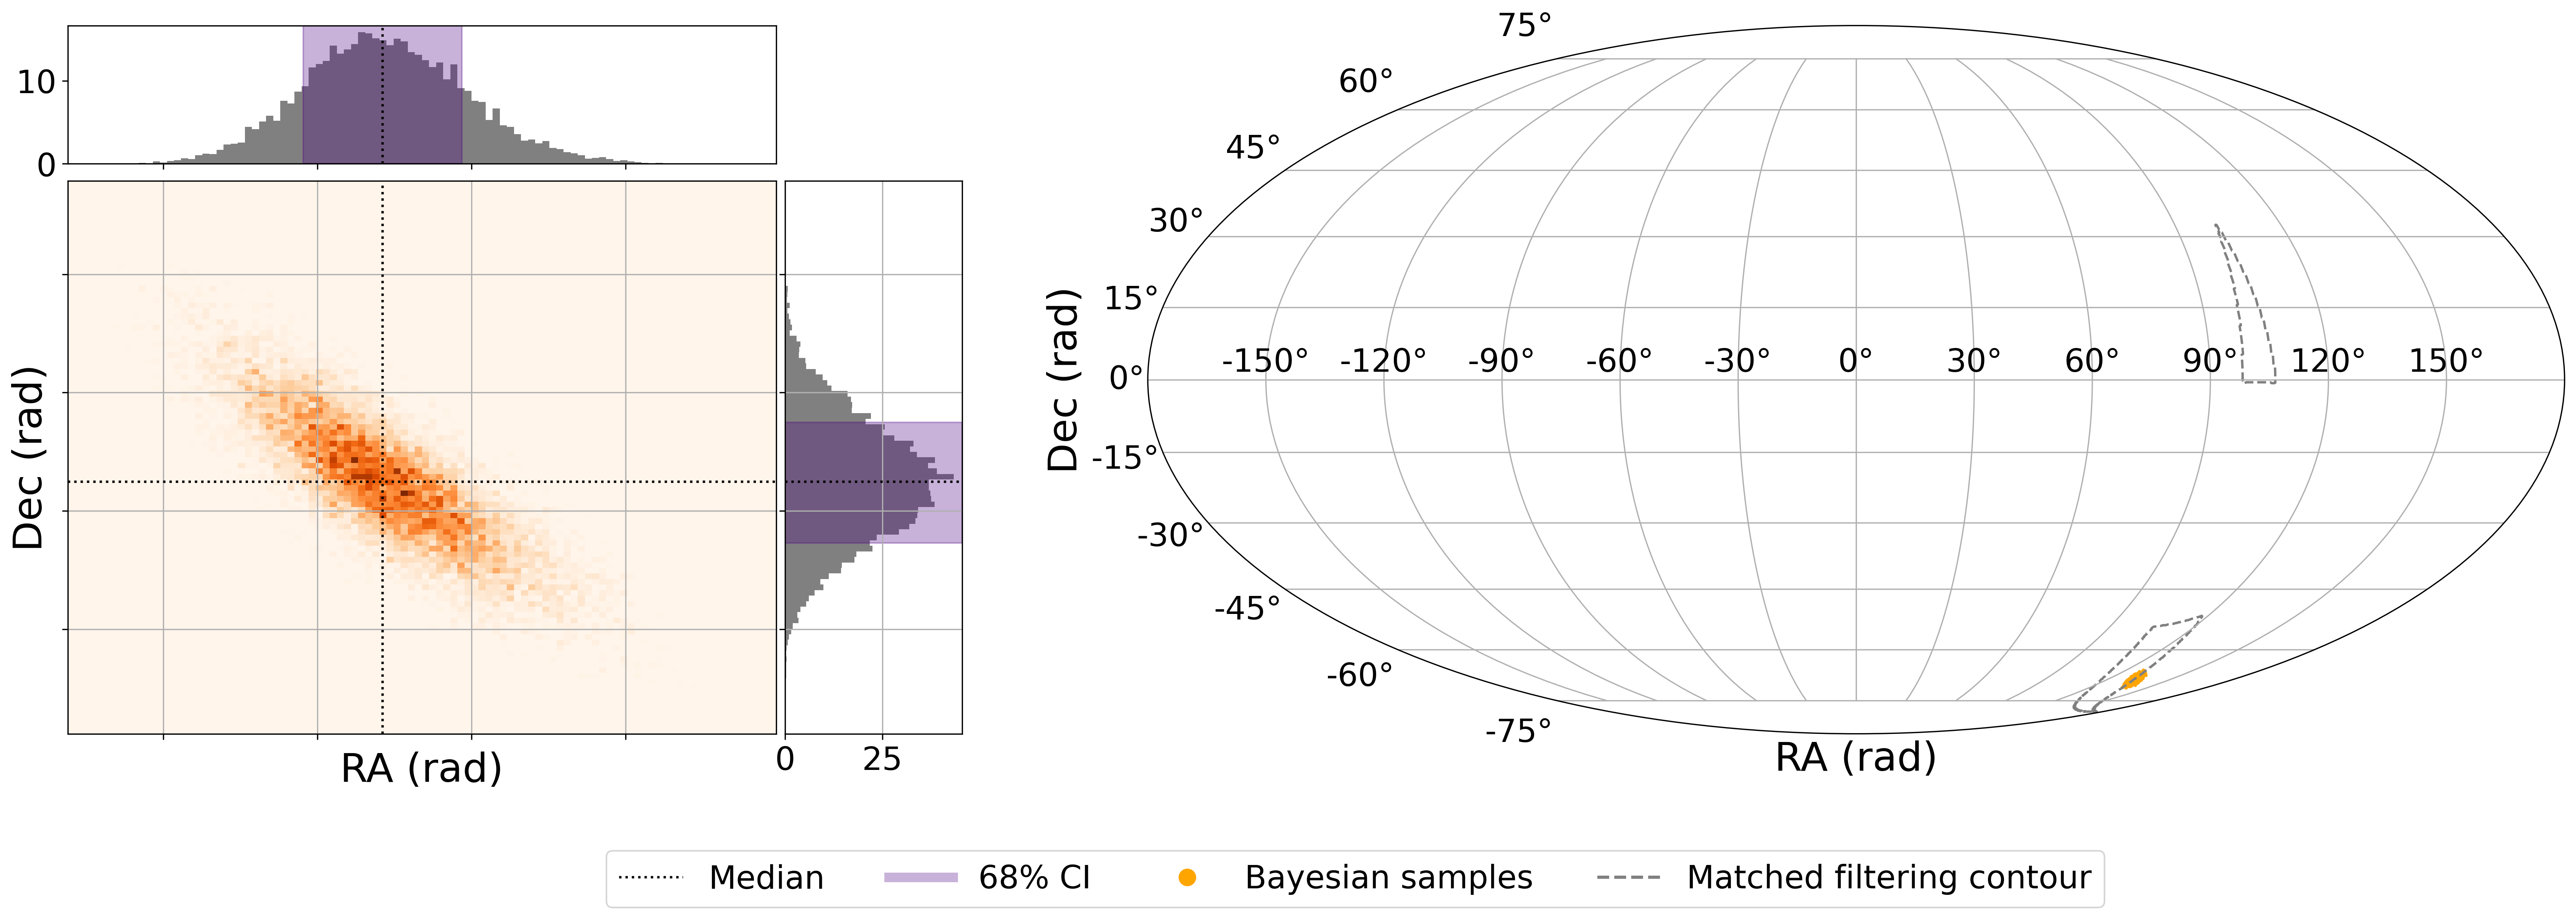
\includegraphics[width=\columnwidth, keepaspectratio]{../figures/radec_posterior_HLV.png}
    \caption{Left: RA and Dec posterior distribution from the Bayesian inference method with 1D marginalisations of the RA and Dec coordinates. The shaded area (purple) indicates the 68\% credible interval while the dotted lines indicate the median of both the RA and Dec distributions. Right: Comparison of the posterior distribution of the RA and Dec coordinates from the Bayesian inference method to the matched filtering method. The grey contour shows the matched filtering enclosed area while the orange scatter points show the posterior distribution from the Bayesian inference method. The blue star indicates the median location of the source.}
    \label{fig:hlv_compare}
\end{figure}

\begin{figure}
    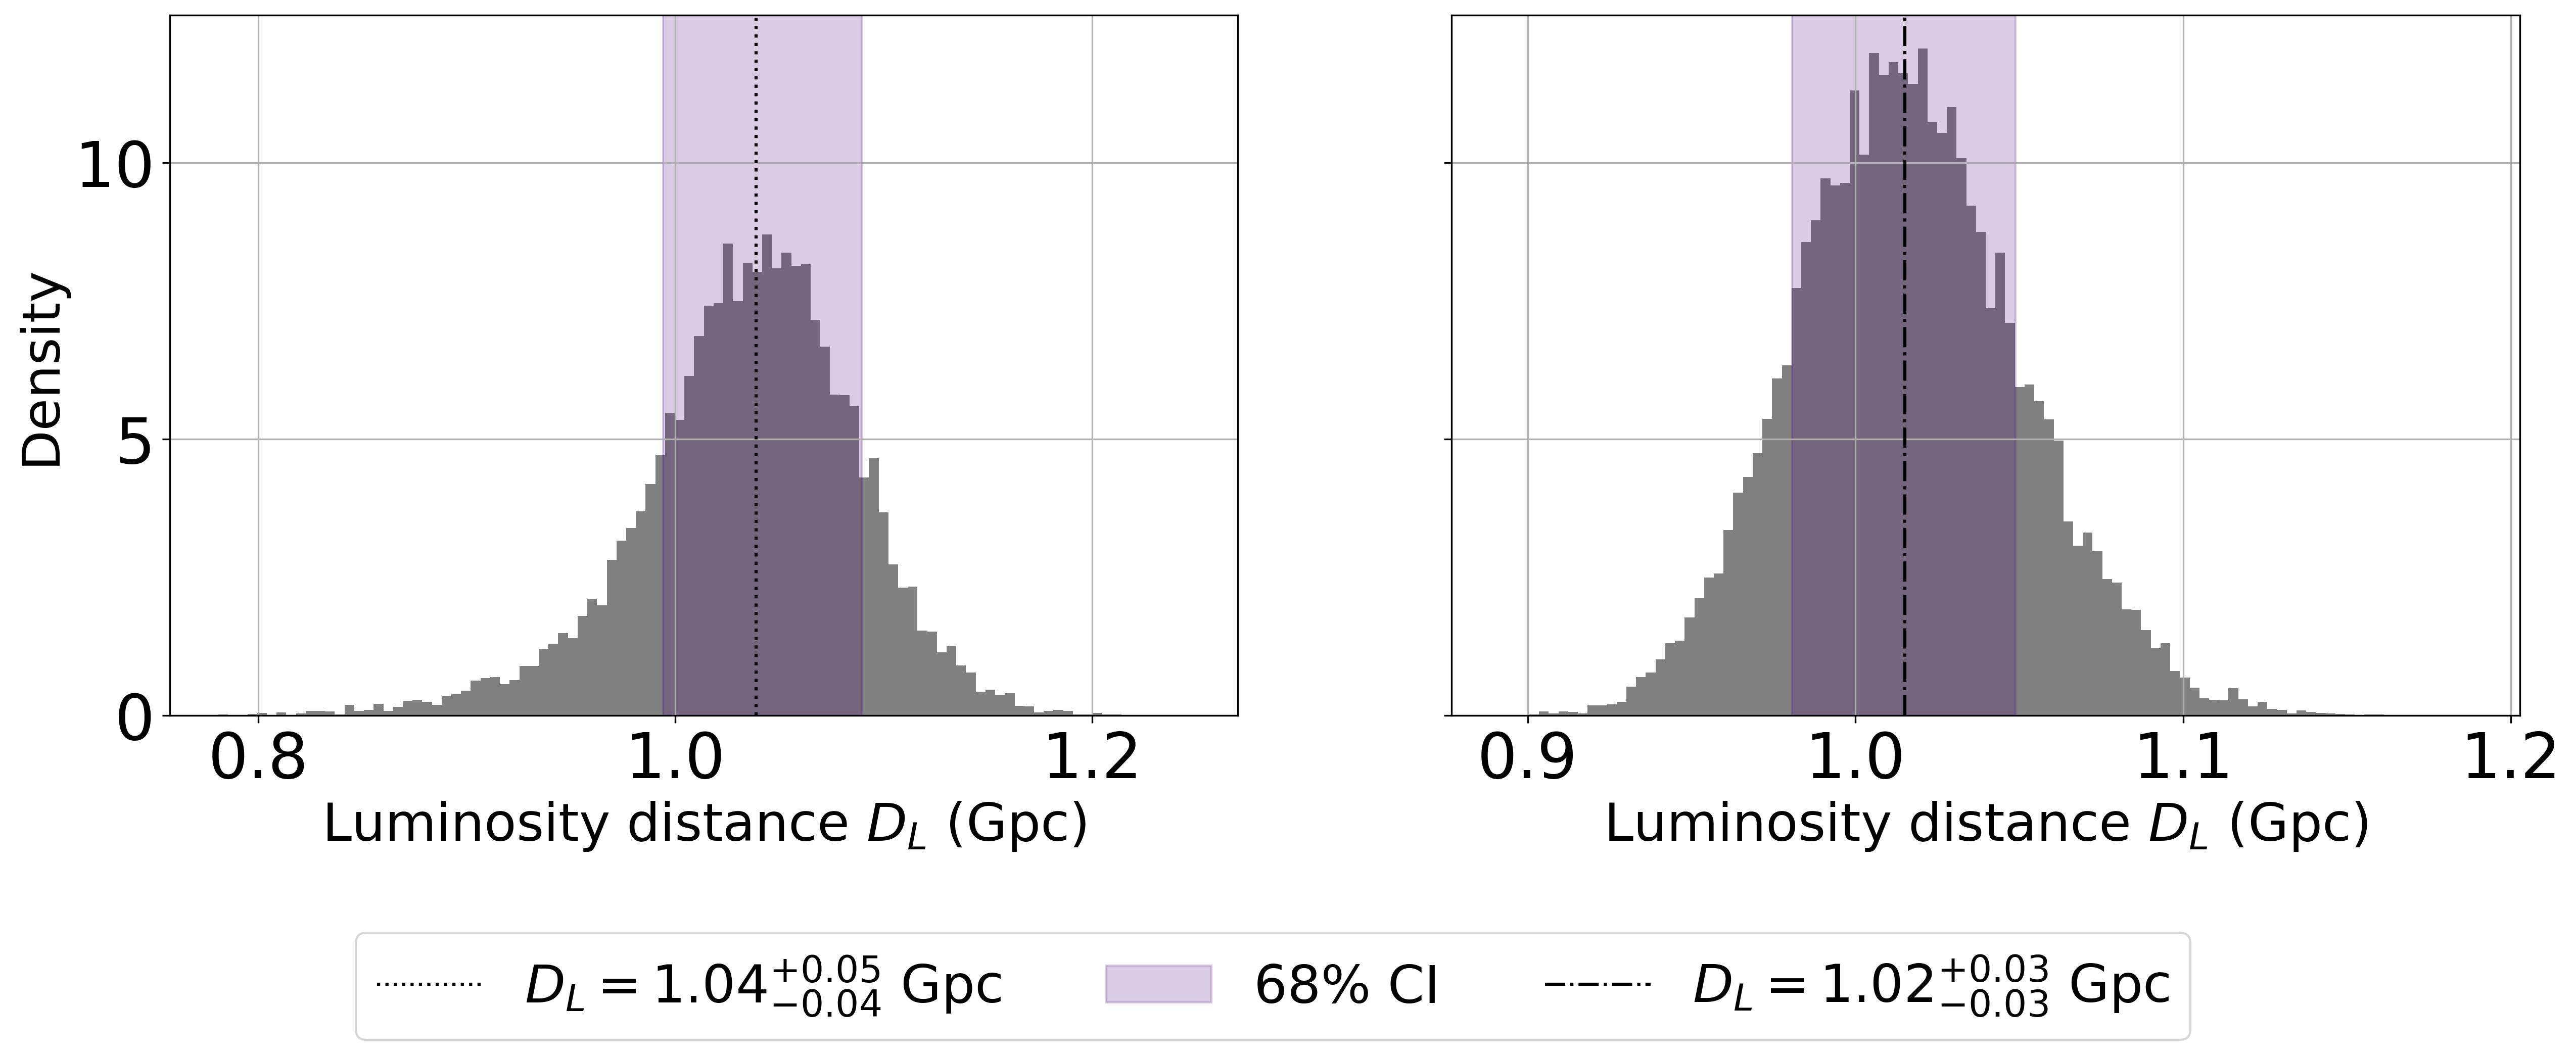
\includegraphics[width=\columnwidth, keepaspectratio]{../figures/dl_posterior.png}
    \caption{Left: Posterior distribution of the luminosity distance $D_L$ for the HL interferometer pair. Right: Posterior distribution for the luminosity distance $D_L$ including the Virgo V1 interferometer. The shaded area (purple) indicates the 68\% credible interval while the dotted lines indicate the median of the distribution. The vertical lines indicate the 5th, 50th (median), and 95th percentiles of the distribution. The median luminosity distance is $1.02 \pm 0.03$ Gpc for both cases.}
    \label{fig:luminosity_distance}
\end{figure}

\begin{table}[h]
    \centering
    \begin{tabular}{c|c|c|c}
    Method & Interferometers & Sky area (deg$^2$) & Improvement\\
    \hline
    Matched filtering & H1 \& L1 & 8472.82 & - \\
    Matched filtering & H1 \& L1 \& V1 & 351.39 & 95.85\% \\
    Bayesian inference & H1 \& L1  & 93.16 & 98.90\% \\
    Bayesian inference & H1 \& L1 \& V1 & 5.04 & 99.94\% \\
    \end{tabular}
    \caption{Summary of the sky areas for the matched filtering and Bayesian inference methods for both the HL and HLV interferometer pairs. The improvement over the HL pair matched filtering method is also shown.}
    \label{tab:areas}
\end{table}

\begin{table}[h]
    \centering
    \begin{tabular}{c|c|c}
    Parameter & \multicolumn{2}{c}{Interferometers} \\
    & H1 \& L1 & H1 \& L1 \& V1 \\
    \hline
    RA ($\alpha$, rad) & $2.477^{+0.164}_{-0.510}$ & $2.321^{+0.046}_{-0.041}$ \\
    Dec ($\delta$, rad) & $-1.123^{+0.214}_{-0.137}$ & $-1.195^{+0.017}_{-0.017}$ \\
    Polarisation angle ($\psi$, rad) & $-0.629^{+0.534}_{-0.229}$ & $-0.462^{+0.061}_{-0.064}$ \\
    Geocentric coalescence time ($t_c^{geo}$, s) & $1126259462.4^{+0.002}_{-0.001}$ & $1126259462.4^{+0.00}_{-0.00}$ \\
    Luminosity distance ($D_L$, Gpc) & $1.039^{+0.075}_{-0.095}$ & $1.015^{+0.061}_{-0.054}$ \\
    \end{tabular}
    \caption{Summary of the median and 1$\sigma$ uncertainties for the parameters obtained from the Bayesian inference method for both the HL and HLV interferometer pairs. The RA and Dec are in radians, the polarisation angle is in radians, the geocentric coalescence time is in seconds, and the luminosity distance is in Gigaparsecs.}
    \label{tab:params}
\end{table}
\clearpage
\section{GW Cosmology}
\label{sec:cosmology}
With the median RA and Dec coordinates of the GW source as well as the median luminosity distance $D_L$, it is possible to estimate the Hubble constant $H_0$ using the known redshift $z$ of the host galaxy. 

First, the host galaxy is identified by cross-matching the GW source coordinates with a galaxy catalog, using the 90\% credible region of the 2D RA and Dec posterior distribution as the search area. The galaxies matched using this method are shown in Fig.~\ref{fig:matched_galaxies} and Table~\ref{tab:galaxies}.

\begin{figure}[h]
    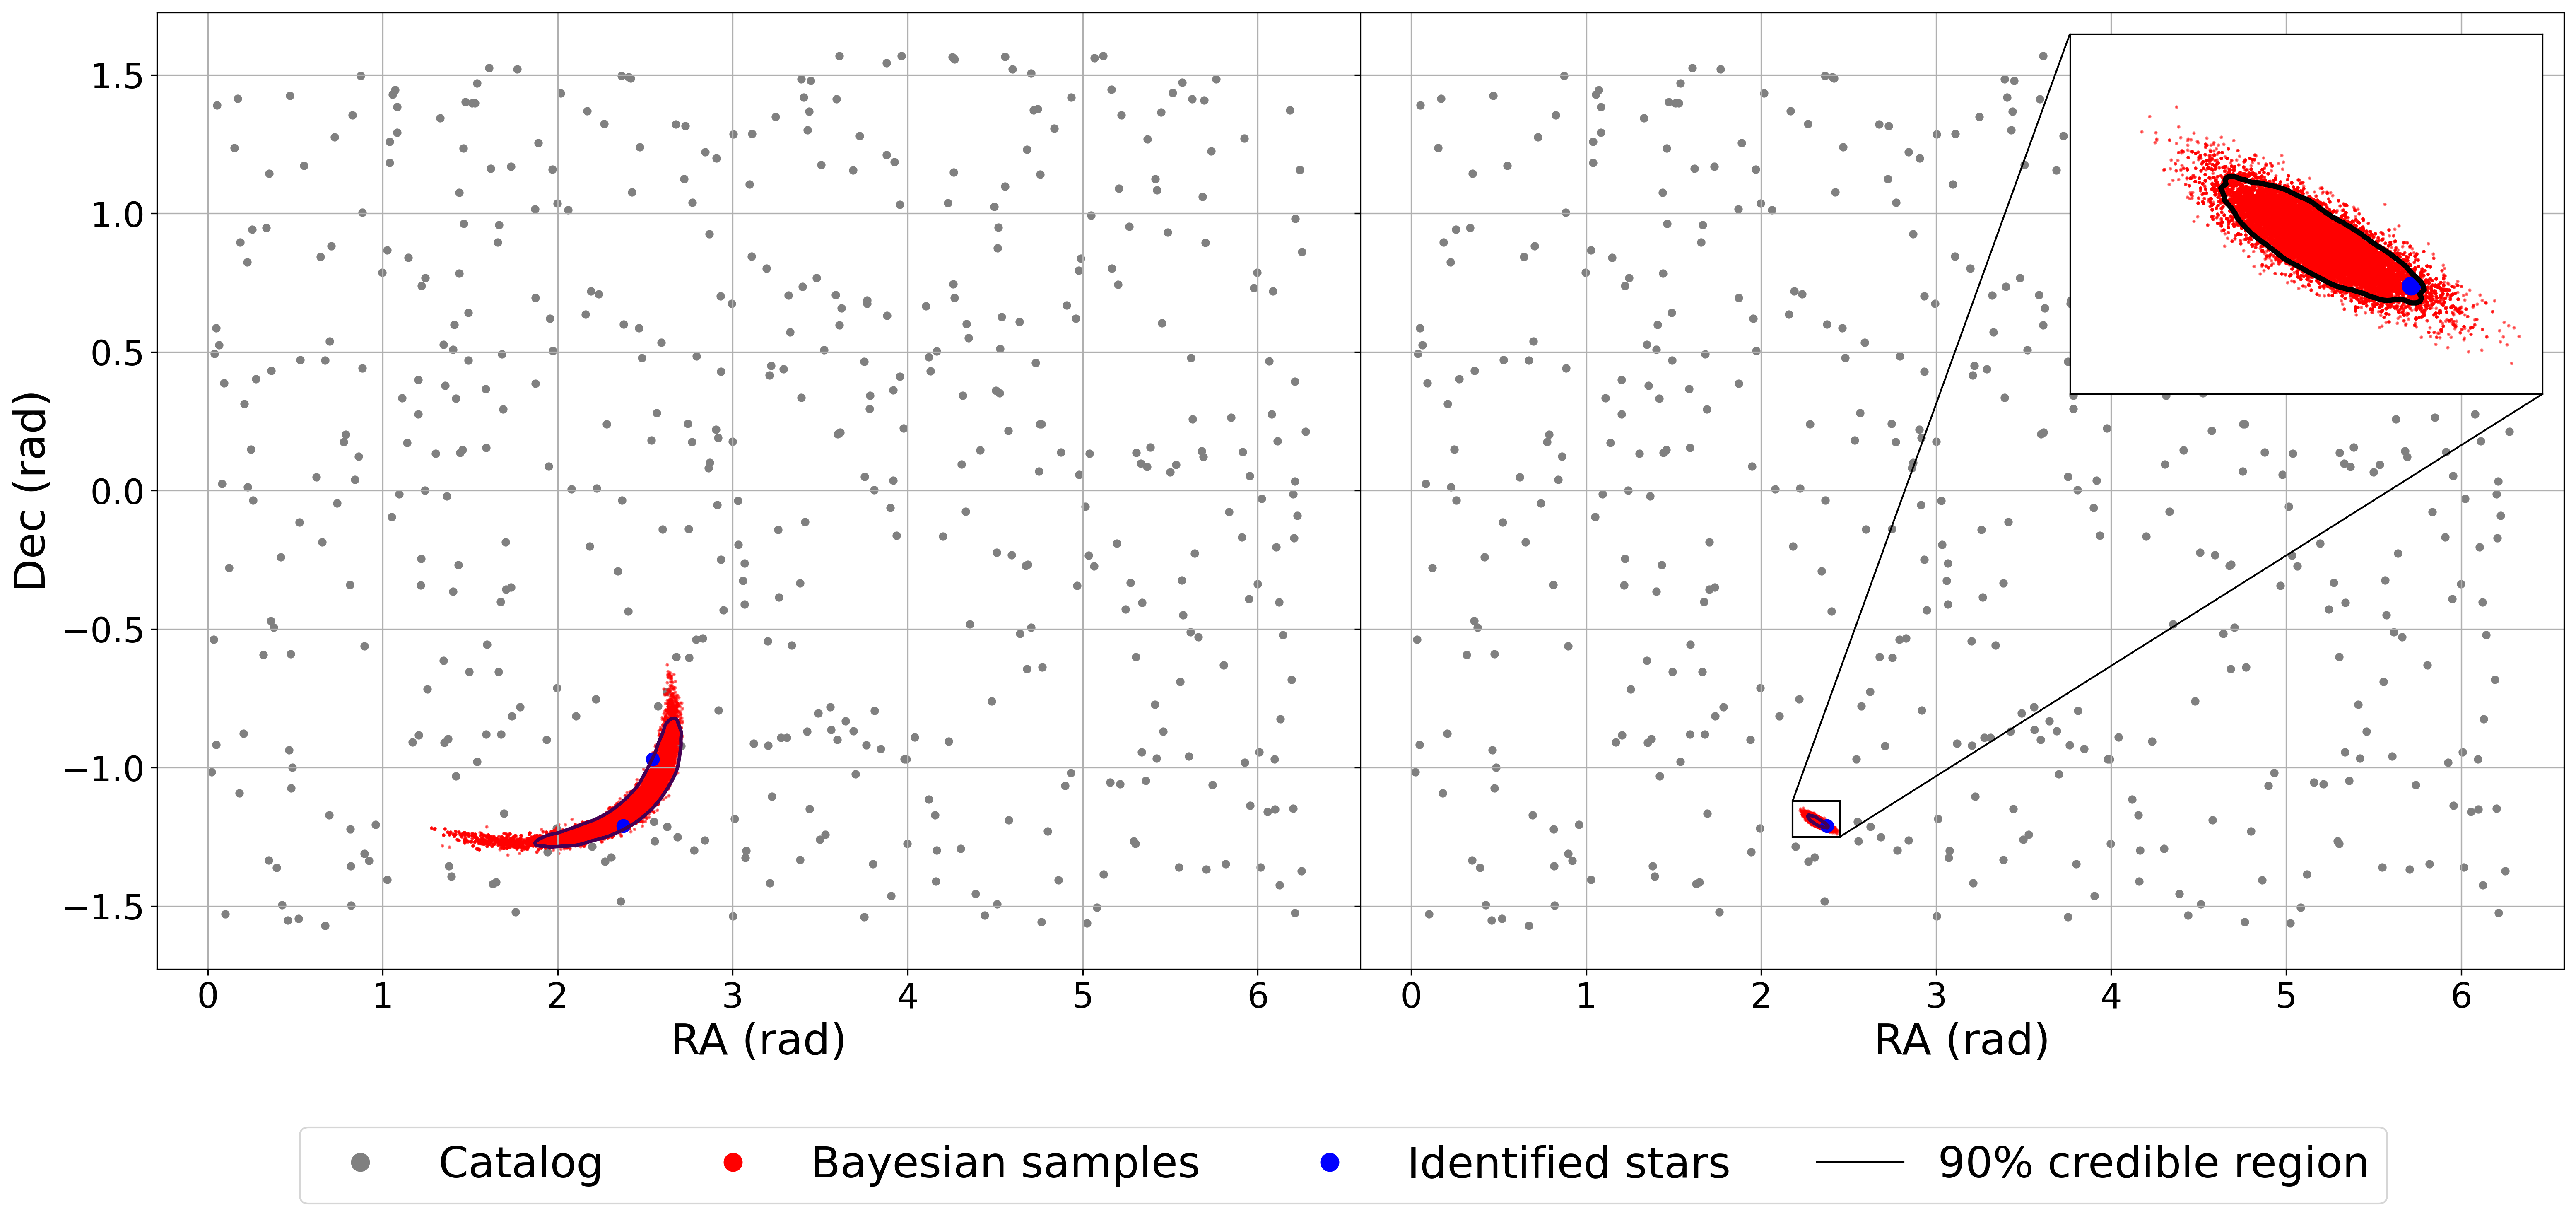
\includegraphics[width=\columnwidth, keepaspectratio]{../figures/kde_crossmatch.png}
    \caption{Left: HL interferometer pair RA and Dec posterior distribution (red) overplotted on catalog distribution of galaxies (grey). The cross-matched galaxies are shown in blue. Right: HLV interferometer pairs RA and Dec posterior distribution (red) overplotted on catalog distribution of galaxies (grey). The cross-matched galaxies are shown in blue. Also shown is a zoomed-in inset of the posterior distribution and cross-matched galaxy in the top right-hand corner.}
    \label{fig:matched_galaxies}
\end{figure}

\begin{table}[h]
    \centering
    \begin{tabular}{c|c|c|c}
    \multicolumn{4}{c}{H1 \& L1 Bayesian inference} \\
    Galaxy & RA (rad) & Dec (rad) & Redshift ($z$) \\
    \hline
    MGC+JGS5HZS & $2.543$ & $-0.969$ & 0.797 \\
    MGC+JN7U119 & $2.375$ & $-1.211$ & 0.226 \\
    \hline
    \multicolumn{4}{c}{H1 \& L1 \& V1 Bayesian inference} \\
    Galaxy & RA (rad) & Dec (rad) & Redshift ($z$) \\
    \hline
    MGC+JN7U119 & $2.375$ & $-1.211$ & 0.226 \\
    \end{tabular}
    \caption{Host galaxies matched to the GW source coordinates using the 90\% credible region of the 2D RA and Dec posterior distribution. The RA and Dec are in radians, and the redshift is dimensionless.}
    \label{tab:galaxies}
\end{table}

As only one galaxy was matched for the H1 \& L1 \& V1 interferometer pair, there was no need to rank the galaxies by likelihood of being the host galaxy. 

Assuming that MGC+JN7U119 is the host galaxy, the redshift $z$ of the host galaxy is 0.226. Using this redshift as well as the median luminosity distance $D_L = 1.02 \pm 0.03$ Gpc from the H1 \& L1 \& V1 Bayesian inference method, the Hubble constant $H_0$ (km/s/Mpc)can be estimated using the following Eq.~\ref{eq:hubble}:

\begin{equation}
    H_0 = \frac{c}{D_L}{z},
    \label{eq:hubble}
\end{equation}
where $c$ is the speed of light in vacuum in km/s, $D_L$ is the luminosity distance in Megaparsecs, and $z$ is the redshift of the host galaxy. Using Eq.~\ref{eq:hubble} results in a Hubble constant $H_0=66.74^{+2.35}_{-2.14}$ km/s/Mpc. 

Additionally, the Hubble constant can also be calculated by inverting Eq.~\ref{eq:hubble2}:
\begin{equation}
    D_L(z) = \frac{c(1 + z)}{H_0} \int_0^z \frac{dz'}{\sqrt{\Omega_m (1 + z')^3 + \Omega_\Lambda + \Omega_\mathrm{rel}(1+z')^4}},
    \label{eq:hubble2}
\end{equation}

which results in a Hubble constant $H_0=77.90^{+2.74}_{-2.50}$ km/s/Mpc.

\clearpage
\section{Conclusion}
\label{sec:conclusion}
In conclusion, matched filtering and Bayesian inference can be used to characterise the GW source depending on which interferometers are used and how many are used. The choice of interferometers is important because their geographic locations and configurations impact the recorded coalescence times as well as which sky sensitivity patterns. This then allows for tighter constraints on the GW source location as well as the luminosity distance, polarisation angle, and geocentric coalescence time. 

Additionally, Bayesian inference, while slower, tends to be able to constrain the GW source location parameters more effectively than matched filtering, even with fewer interferometers used. This is because the goal of matched filtering is to detect a GW signal in the data with use of a known template which is modulated by the antenna response of the interferometers. The modified template that maximises the SNR is the best match, with the assumption that the original template was a good approximation of the true GW signal and the RA, Dec, and $\psi$ parameters given to the antenna response function are close to the true values. This best match gives the coalescence time $t_c$ for each interferometer, which is then used to calculate the time delays between the interferometers and the geocenter. The time delays are then used to create a sky map of the likely area the GW source is located in. However, the matched filtering method cannot constrain the luminosity distance $D_L$ and geocentric coalescence time $t_c^{geo}$ parameters and only provides point estimates for $\alpha, \delta$ and $\psi$. In contrast, Bayesian inference uses the likelihood function shown in Eq.~\ref{eq:likelihood} to calculate the posterior distributions over all the parameters. This allows for all the parameters to be constrained simultaneously, especially with the addition of the Virgo V1 interferometer.

The results of the analysis show that the GW signal, when considering all three interferometers, is likely located at ($2.32^{+0.05}_{-0.04}$, $-1.20^{+0.02}_{-0.02}$) in host galaxy MGC+JN7U119 with a luminosity distance of $1.02 \pm 0.03$ Gpc. This host galaxy has a redshift at a redshift of 0.226, which allows to estimate the Hubble constant to be $H_0=66.74^{+2.35}_{-2.14}$ km/s/Mpc using the Hubble Law $H_0=v/D_L$ shown in Eq.~\ref{eq:hubble}, where $v\simeq cz$. The Hubble constant can also be estimated to be $H_0=77.90^{+2.74}_{-2.50}$ km/s/Mpc by inverting Eq.~\ref{eq:hubble2}.

\clearpage
\bibliographystyle{vancouver-authoryear}
\bibliography{bibliography}
\appendix
\section{Use of auto-generation tools}
Auto-generation tools were used to help parse error messages throughout the project, and to help format this \LaTeX\ report as well as adding doctrings to the functions. Autogeneration tools were used in Section~\ref{sec:cosmology} when creating the code to invert Eq.~\ref{eq:hubble2}.

Auto-generation tools were not used elsewhere, for code generation, writing, or otherwise.
\end{document}